\documentclass[twoside,a4paper]{article}
\usepackage{geometry}
\usepackage{booktabs}
\usepackage{tabu}
%for some reason the compiler kills itself with {comment} package
\newgeometry{
  top=0.75in,
  bottom=0.75in,
  outer=1in,
  inner=1in,
}
\usepackage{graphicx}
\usepackage{amsmath}
\usepackage{siunitx}
\usepackage{cancel}
\usepackage{float}
\usepackage[
backend=biber,
style=numeric,
sorting=none
]{biblatex}

\addbibresource{mybibliography.bib}
\title{Report 1: }
\title{\textbf{FIT: Report 1} \\[1ex] \Large \underline{Handwriting detection and Note Conversion using OCR}
}
\author{Pietka Ł, Barot H, Krzyszosiak M, Markowicz J, Milewski M, Sobczak M}
\date{March 12 2025}
\begin{document}
\maketitle
\tableofcontents
\newpage
\section{Re-evaluating Report 1}

In report 1, the aim of the project was stated to be creation of  a program that utilizes OCR technology, which allows for recognition and digitization of handwritten notes 
into easily readable and storable text documents on a computer. However, the project was not clearly defined and the problem statement was not well articulated.
The target population was not specified, and the aim of the project was not clearly defined. The project lacked a clear focus and direction, which made it difficult to understand the purpose and goals of the project.

Due to the target population being vague, multiple areas of this project were hard to define, and ambiguous as to what direction the project is headin in.
This was a major roadblock because when we discussed questions like "Do the samples include math equations?" or "Do the samples include letters?" "Are the letters allowed to be geometrically malformed or the the samples have to be
clean and perfectly written?". Our group memmbers had different approaches to these questions, and this led to a lot of confusion and miscommunication.

Hence, this report would like to revisit and address the flawed initial approach. Define the who the project is for, which will make it simpler to find source of raw data,
and implement a model that will best suit the use case defined.

\subsection{Problem Statement}
Certain two members of our group particularly enjoyed writting english literature. Wether it was analitical essays, or fantasy stories. They both agreed that writting on a physical paper felt the most comfortable and natural. However, they couldn't organize their raw notes and digitizing them was 
really time consuming. Hence, we decided to create a program that would help them with this problem. The specific aim of this project is to create a program
for the the two members of our group, that could assist in digitization of their english literature notes.

\section{Data Collection Procedure: }
In the previous report, we decided to use the GNHK dataset~\cite{Lee2021}, as it best suited the freely available OCR model that we chose. However, this was a large dataset, that contained
a variety of different samples. The sample types included math equations, plain english text, distorted handwritting and much more. Additionally these datasets conainted a the different types of english (british, american, asian) used all over the world.

This essentially ment, that this dataset ranged over a wider domain than what was needed for our project. This is displayed using 
a venn diagram in figure~\ref{fig:venn_diagram}. Set A (red circle) is the collectioon of what GNHK has to offer, meanwhile Set B (blue circle) is
what is required for our project. The intersection of the two sets is what we need.
\begin{figure}[H]
  \centering
  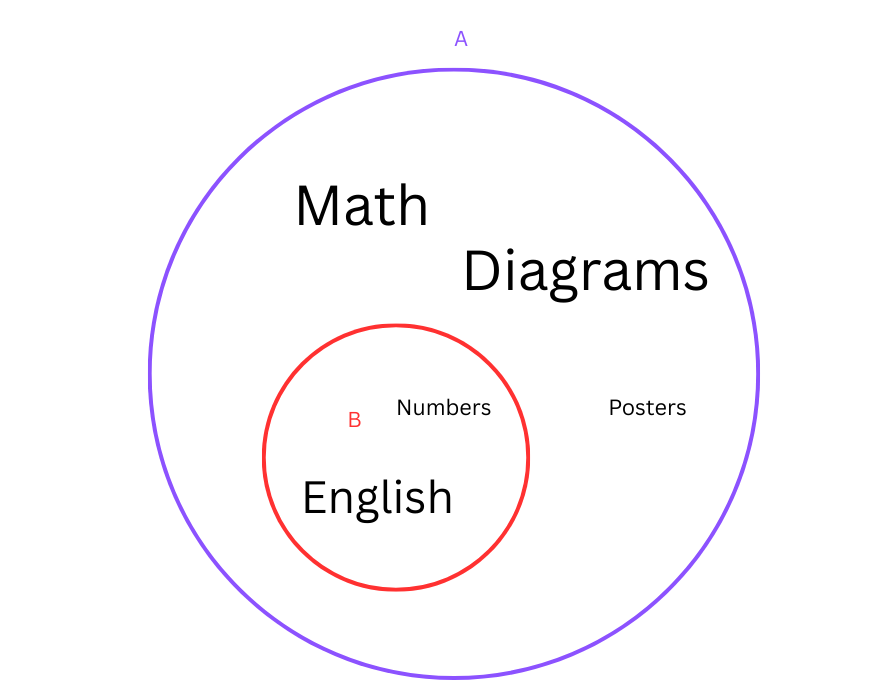
\includegraphics[width=0.8\textwidth]{VennDiagram_WhatWeNeed.png}
  \caption{Venn Diagram of Dataset Characteristics vs. Project Needs}
  \label{fig:venn_diagram}
\end{figure}

To collect the data we had two choices: 
\begin{enumerate}
  \item We could have used the GNHK dataset, and filtered out the samples that we did not need. However, this would be a time consuming process, and we would have to manually go through each sample.
  \item The target population (two writters) are asked to send samples of their handwritting, of this exact same sentence. 
\end{enumerate}

We decided to go with the second option, as it would be much easier to collect and it would be more represntative of the target population's needs.
The sentence chosen was "The quick brown fox jumps over the lazy dog". This sentence was chosen because it contains all the letters of the english alphabet, and it is a common pangram used in handwriting samples.
Additionally, the users were asked to write this sentence in all lowercase or uppercase, alternating between them. They were also asked to number each line, to get alphanumeric data.
\section{Raw Data (samples and syntatic characteristics): }

\section{Normalization of Raw Data: }
\section{Extraction of words/letters: }
\section{Closing Thoughs: }
\printbibliography
\end{document}